\chapter{Εισαγωγή}
\label{chap1}

%Εδώ αυτή κάνουμε μια γενική περιγραφή του χώρου εφαρμογής της διπλωματικής. Αναφέρουμε τα χαρακτηριστικά του χώρου και καταλήγουμε στα γενικότερα προβλήματα που αντιμετωπίζει ο χώρος. Η συζήτηση των προβλημάτων θα πρέπει να προϊδεάζει τον αναγνώστη για το τι θα προσπαθήσει να αντιμετωπίσει η διπλωματική, χωρίς ακόμα να αναφερόμαστε συγκεκριμένα στο αντικείμενο της διπλωματικής.
Είναι ευρεώς διαδεδομένο πως η ψηφιακή ενημέρωση βαδίζει πλέον με ραγδαίους ρυθμούς. Αμέτρητοι είναι σήμερα οι ιστότοποι και διαδικτυακές κοινότητες που σχετίζονται με όλες τις εκφάνσεις της καθημερινότητας, καθώς νέες εφαρμογές ενημέρωσης, οργάνωσης και επικοινωνίας αναδύονται στην ψηφιακή αγορά καθημερινά. Με μια αναζήτηση στο διαδίκτυο, ή με μια επισήμανση εντός της εφαρμογής, ο χρήστης μπορεί να ενημερωθεί για γεγονότα που τον ενδιαφέρουν, να δεχθεί ειδοποιήσεις για εκδηλώσεις που τον αφορούν, ή ακόμη και να προγραμματίσει το δρομολόγιό του, να υπολογίσει χρονικές και οικονομικές μεταβλητές και να σχεδιάσει το πλάνο του. Είναι λοιπόν ευνόητο το πρόβλημα που ανακύπτει από το παραπάνω φαινόμενο, σχετικά με την επικαιροποίηση και ενημέρωση της πληροφορίας που παρέχεται στο χρήστη. Παράγοντες όπως κυκλοφοριακή συμφόρηση, καιρικές αντιξοότητες, καθυστέρηση έναρξης της διοργάνωσης ή άφιξης των συμμετεχόντων και άλλες αναπάντεχες εκβάσεις είναι αδύνατο να συνυπολογιστούν με κάποιον αλγόριθμο στις προαναφερθείσες εφαρμογές.

Από την άλλη, η απότομη στροφή των εφαρμογών και των μέσων κοινωνικής δικτύωσης γύρω από την ατομικότητα, έχει ως αντίκτυπο την αποδυνάμωση του \textit{κοινωνικού γίγνεσθαι}. Πλέον είναι προτιμότερη η απομακρυσμένη έμμεση επικοινωνία με μέσα που τροφοδοτούν το χρήστη με εγωπαθή συμπτώματα και τον απομακρύνουν από την πραγμαματική έννοια της επικοινωνίας. Συχνό είναι επίσης το φαινόμενο εκμετάλλευσης της κοινωνικής προβολής για επαγγελματική ανέλιξη. Εντούτοις, λόγοι με πολιτισμικό υπόβαθρο περνάνε σε δεύτερη μοίρα (βλ. Σχ \ref{socialmediausage}). 

Σαν αποτέλεσμα, τόποι κοινωνικού και πολιτισμικού περιεχομένου επισκιάζονται από αυτές τις εφαρμογές ``\textit{γίγαντες}'' (\selectlanguage{english}\textit{facebook, instagram, snapchat, twitter, tinder}\selectlanguage{greek} κλπ.). Εκδηλώσεις που χρήζουν προσοχής καταλήγουν να μην δέχονται την κατάλληλη προβολή. Είναι επομένως επιτακτική η ανάγκη ευαισθητοποίησης του χρήστη προκειμένου να δράσει υπερ του προσωπικού, αλλά τατοχρόνως και κοινωνικού οφέλους.   

\begin{figure}[!t]
	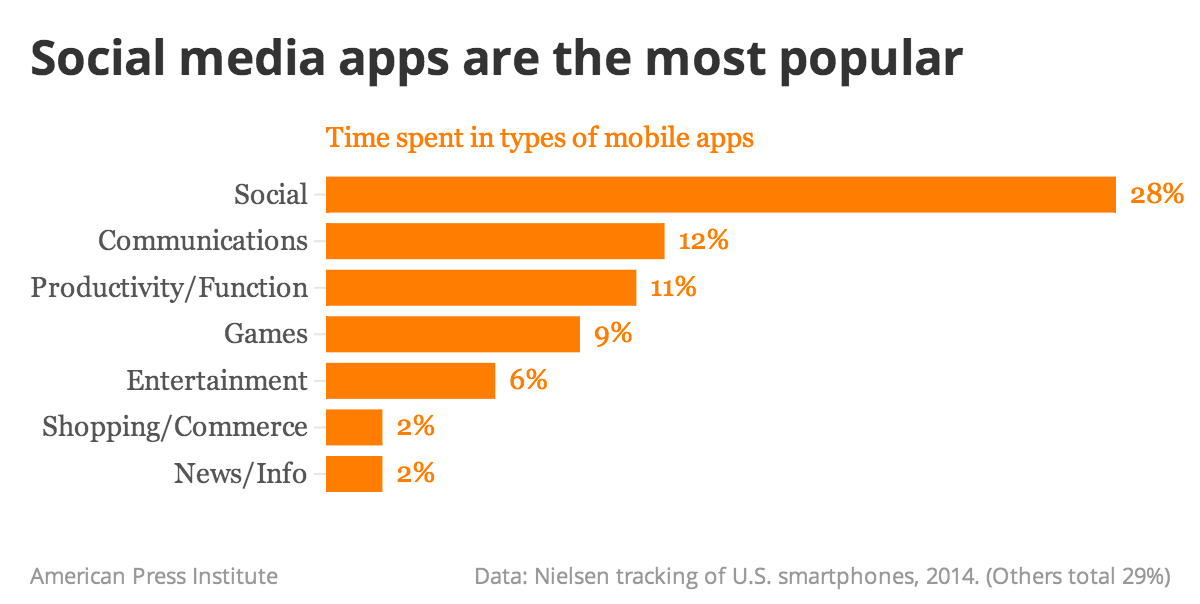
\includegraphics[scale=0.3]{figures/social-media-usage.png}
	\centering
	\caption{Οι χρήστες ξοδεύουν 14 φορές περισσότερο χρόνο χρησιμοποιώντας εφαρμογές όπως το \selectlanguage{english} \textit{facebook}\selectlanguage{greek}, έναντι εφαρμογών ενημέρωσης  (Πηγή: \cite{[AMP+14]})}
	\label{socialmediausage}
\end{figure}



\section{Αντικείμενο της διπλωματικής}

Εδώ αναφερόμαστε συγκεκριμένα στο τί θα κάνει η διπλωματική. Αναφέρουμε λεπτομερώς α) τα προβλήματα που θα λύσει (και που ήδη έχουν περιγραφεί γενικά στην προηγούμενη ενότητα), και β) πώς σκοπεύει να τα λύσει. 
Είναι σημαντικό κάποιος που θα διαβάσει την ενότητα αυτή να καταλάβει σε σημαντικό βαθμό τον σκοπό της διπλωματικής σας και τις τεχνικές δυσκολίες της, χωρίς να είναι αναγκαίο να δει όλα τα άλλα κεφάλαια. Η ενότητα αυτή θέλει πολύ προσοχή και καλύτερα να τη γράψετε αφού έχετε γράψει όλα τα υπόλοιπα κεφάλαια.

Το αντικείμενο με το οποίο καταπιάνεται το παρόν έργο, επικεντρώνεται στην σχεδίαση και την υλοποίηση μιας εφαρμογής, βασισμένη στην πρακτική ενεργοποίησης ενός ``\textit{πλήθους}'' ή μιας ομάδας, γνωστής και ως \textit{τακτική του πληθοπορισμού}. 

\subsection{Συνεισφορά}
Εδώ παραθέτουμε αριθμητικά συγκεκριμένες ενέργειες/λύσεις/μεθοδολογίες που παρουσιάζει η διπλωματική και λύνουν τα προβλήματα που υποσχεθήκαμε στην προηγούμενη ενότητα ότι θα λύσει η διπλωματική. Συνήθως η υποενότητα αυτή έχει την παρακάτω μορφή:

Η συνεισφορά της διπλωματικής συνοψίζεται ως εξής:
\begin{enumerate}
\item Μελετήθηκαν συστήματα κ.λ.π.
\item Υλοποιήθηκαν τρεις αλγόριθμοι υπολογισμού κ.λ.π.
\item Αξιολογήθηκε η επίδοση των αλγορίθμων και βρέθηκε ότι κ.λ.π.
\item Ενσωματώθηκαν οι αλγόριθμοι σε πρότυπο σύστημα κ.λ.π.
\item ...
\end{enumerate}


\section{Οργάνωση του τόμου}

Εδώ περιγράφουμε τα κεφάλαια της διπλωματικής: μία πρόταση για το τί θα έχει  κάθε κεφάλαιο.Συνήθως η ενότητα αυτή έχει την παρακάτω μορφή (δεν θα σας πάρει πάνω από μία μεγάλη παράγραφο):

Εργασίες σχετικές με το αντικείμενο της διπλωματικής παρουσιάζονται στο Κεφάλαιο \ref{chap2}. Το Κεφάλαιο \ref{chap3} συζητά θέματα μοντελοποίησης. Στο Κεφάλαιο \ref{chap4} αναπτύσσουμε κ.λ.π. 

Τονίζεται ότι η διάρθρωση του υπόλοιπου κειμένου (πλήθος και έκταση κεφαλαίων), καθώς και η ονομασία κάθε κεφαλαίου ή ενότητας σε αυτό το πρότυπο είναι εντελώς ενδεικτικά. Για την τελική οργάνωση του κειμένου σας, συμβουλευθείτε τον επιβλέποντα της εργασίας.

